\section{Umkehrabbildung}

\textbf{Definition (Umkehrabbildung):}

Seien $D_f$ und $W_f$ Mengen und
$f:D_f\rightarrow W_f$ eine bijektive Abbildung.
Dann gibt es zu jedem $y\in W_f$ genau ein $x\in D_f$
mit $f(x)=y$.

Die Umkehrabbildung ist definiert durch
\[
f^{-1}:W_f\rightarrow D_f,\qquad
y\mapsto x \quad\text{mit } f(x)=y.
\]
Sie wird auch Umkehrfunktion genannt.

Die folgende Zeichnung verdeutlicht die Zuordnung
$x\mapsto f(x)$ und die Rückzuordnung
$y\mapsto f^{-1}(y)$.

\begin{center}
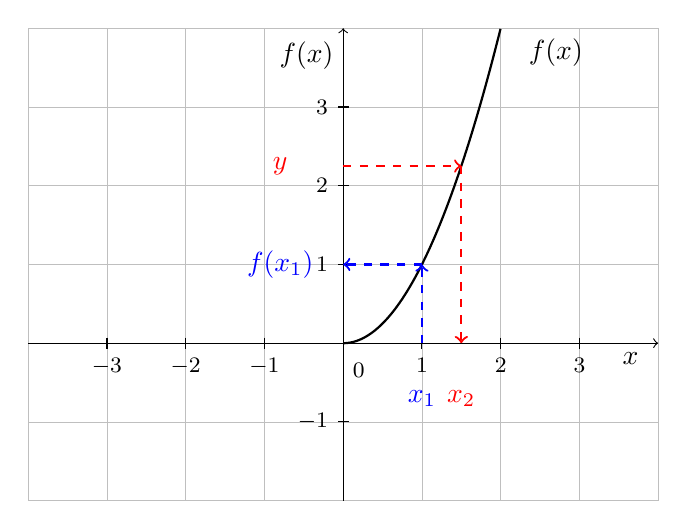
\begin{tikzpicture}
		
		% Gitternetzlinien
		\draw[xstep=1cm, ystep=1cm, very thin, color=lightgray] (-4,4) grid (4,-2);
		% x-Achse
		\draw[->] (-4,0) -- (4,0) node[below,xshift=-1em] {$x$}; 
		%Zahlen auf x-Achse
		\foreach \x in {-3,...,-1}
		\draw[shift={(\x,0)},color=black] (0pt,2pt) -- (0pt,-2pt) node[below] {\footnotesize $\x$};
		\foreach \x in {1,...,3}
		\draw[shift={(\x,0)},color=black] (0pt,2pt) -- (0pt,-2pt) node[below] {\footnotesize $\x$};
		% y-Achse 
		\draw[->] (0,-2) -- (0,4) node[left,yshift=-1em] {$f(x)$};%node[above left]
		%Zahlen auf y-Achse
		\foreach \y in {-1,...,-1}
		\draw[shift={(0,\y)},color=black] (2pt,0pt) -- (-2pt,0pt) node[left] {\footnotesize $\y$};
		\foreach \y in {1,...,3}
		\draw[shift={(0,\y)},color=black] (2pt,0pt) -- (-2pt,0pt) node[left] {\footnotesize $\y$};
		%Ursprung
		\draw[color=black] (0pt,-10pt) node[right] {\footnotesize $0$};
		
		
		
		\draw[thick,color=black] plot[samples=200, domain=0:2] 
		(\x,{\x*\x}) node[below, xshift=2em]{$f(x)$};
		
		\draw[->,color=blue,thick,dashed] (1,0) -- (1,1) ;
		\draw[->,color=blue,thick,dashed] (1,1) --  (0,1) ;
		
		\draw[color=blue,thick,dashed] (1,-0.7) node {$x_1$}  ;
		\draw[color=blue,thick,dashed] (-0.8,1) node {$f(x_1)$}  ;
		
		\draw[->,color=red,thick,dashed] (0,2.25) -- (1.5,2.25) ;
		\draw[->,color=red,thick,dashed] (1.5,2.25) --  (1.5,0) ;
		
		\draw[color=red,thick,dashed] (1.5,-0.7) node {$x_2$}  ;
		\draw[color=red,thick,dashed] (-0.8,2.25) node {$y$}  ;
		
	\end{tikzpicture}
\end{center}

\textbf{Beispiel:}

Wir betrachten die quadratische Funktion mit
eingeschränktem Definitionsbereich:
\begin{align*}
f&:[0,\infty[\ \rightarrow [0,\infty[,
& x&\mapsto x^2,\\
f^{-1}&:[0,\infty[\ \rightarrow [0,\infty[,
& x&\mapsto \sqrt{x}.
\end{align*}

\begin{center}
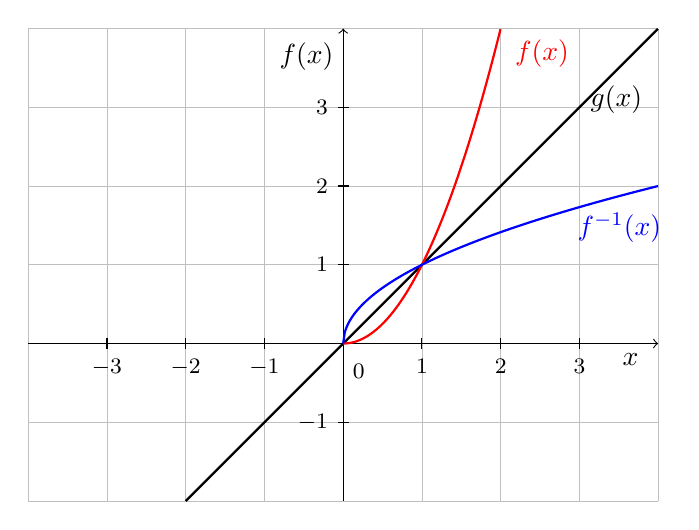
\begin{tikzpicture}
		% Gitternetzlinien
		\draw[xstep=1cm, ystep=1cm, very thin, color=lightgray] (-4,4) grid (4,-2);
		% x-Achse
		\draw[->] (-4,0) -- (4,0) node[below,xshift=-1em] {$x$}; 
		%Zahlen auf x-Achse
		\foreach \x in {-3,...,-1}
		\draw[shift={(\x,0)},color=black] (0pt,2pt) -- (0pt,-2pt) node[below] {\footnotesize $\x$};
		\foreach \x in {1,...,3}
		\draw[shift={(\x,0)},color=black] (0pt,2pt) -- (0pt,-2pt) node[below] {\footnotesize $\x$};
		% y-Achse 
		\draw[->] (0,-2) -- (0,4) node[left,yshift=-1em] {$f(x)$};%node[above left]
		%Zahlen auf y-Achse
		\foreach \y in {-1,...,-1}
		\draw[shift={(0,\y)},color=black] (2pt,0pt) -- (-2pt,0pt) node[left] {\footnotesize $\y$};
		\foreach \y in {1,...,3}
		\draw[shift={(0,\y)},color=black] (2pt,0pt) -- (-2pt,0pt) node[left] {\footnotesize $\y$};
		%Ursprung
		\draw[color=black] (0pt,-10pt) node[right] {\footnotesize $0$};
		\draw[thick,color=black] plot[samples=200, domain=-2:4] 
		(\x,{\x}) node[below, xshift=-1.5em,yshift=-1.7em]{$g(x)$};
		
		\draw[thick,color=red] plot[samples=200, domain=0:2] 
		(\x,{\x*\x}) node[below, xshift=1.5em]{$f(x)$};
		\draw[thick,color=blue] plot[samples=200, domain=0:4] 
		(\x,{sqrt(\x)}) node[below, xshift=-1.4em,yshift=-.6em]{$f^{-1}(x)$};
	\end{tikzpicture}
\end{center}

\textbf{Eigenschaften:}

Für eine bijektive Funktion gelten die Identitäten
\begin{align*}
(f^{-1}\circ f)(x)&=x
&&\text{für alle }x\in D_f,\\
(f\circ f^{-1})(y)&=y
&&\text{für alle }y\in W_f.
\end{align*}

Die Graphen von $f$ und $f^{-1}$ sind bei reellen
Funktionen Spiegelbilder an der Geraden $y=x$,
sofern beide Graphen in demselben Koordinatensystem
dargestellt werden.

Für das Beispiel $f(x)=x^2$ mit $x\geq 0$ folgt:
\begin{align*}
(f^{-1}\circ f)(x)
&=\sqrt{x^2}=|x|=x
&&\text{für }x\geq 0,\\
(f\circ f^{-1})(y)
&=(\sqrt{y})^2=y
&&\text{für }y\geq 0.
\end{align*}

\textbf{Wichtig:}
Die Umkehrfunktion $f^{-1}$ ist nicht mit der
Kehrwertfunktion $1/f(x)$ zu verwechseln.
Außerdem ist das Urbild $f^{-1}(V)$ einer Menge $V$
auch ohne Umkehrfunktion definiert; die Notation
wird aus dem Zusammenhang unterschieden.

\subsection{Aufgabe zur Umkehrabbildung Teil I}

\textbf{Aufgabe:}

Gegeben ist $f(x)=x^2-2x$.

\begin{enumerate}
\item[(i)] Bestimme möglichst große Intervalle,
auf denen $f$ injektiv und somit bei geeigneter
Zielmenge umkehrbar ist.
\item[(ii)] Bestimme die Umkehrfunktion für
die Einschränkung auf $]-\infty,1]$.
\end{enumerate}

\textbf{Lösung zu (i):}

Durch quadratische Ergänzung ergibt sich:
\[
f(x)=x^2-2x=(x-1)^2-1.
\]
Die Parabel hat ihren Scheitelpunkt bei $(1,-1)$
und die Nullstellen $x=0$ und $x=2$.

\begin{center}
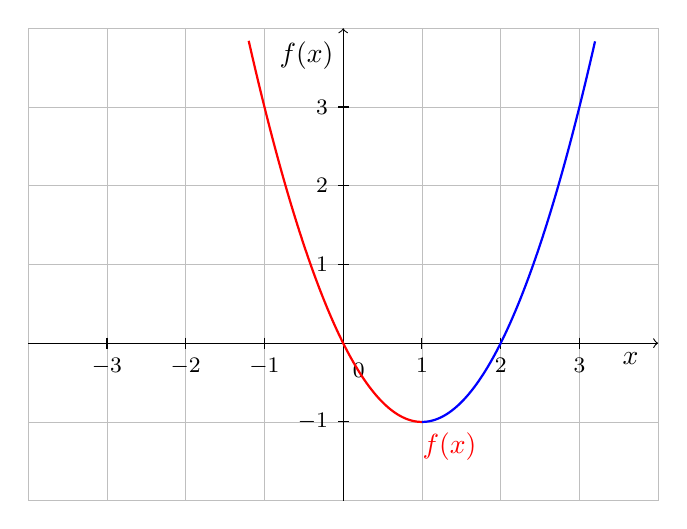
\begin{tikzpicture}
			
			% Gitternetzlinien
			\draw[xstep=1cm, ystep=1cm, very thin, color=lightgray] (-4,4) grid (4,-2);
			% x-Achse
			\draw[->] (-4,0) -- (4,0) node[below,xshift=-1em] {$x$}; 
			%Zahlen auf x-Achse
			\foreach \x in {-3,...,-1}
			\draw[shift={(\x,0)},color=black] (0pt,2pt) -- (0pt,-2pt) node[below] {\footnotesize $\x$};
			\foreach \x in {1,...,3}
			\draw[shift={(\x,0)},color=black] (0pt,2pt) -- (0pt,-2pt) node[below] {\footnotesize $\x$};
			% y-Achse 
			\draw[->] (0,-2) -- (0,4) node[left,yshift=-1em] {$f(x)$};%node[above left]
			%Zahlen auf y-Achse
			\foreach \y in {-1,...,-1}
			\draw[shift={(0,\y)},color=black] (2pt,0pt) -- (-2pt,0pt) node[left] {\footnotesize $\y$};
			\foreach \y in {1,...,3}
			\draw[shift={(0,\y)},color=black] (2pt,0pt) -- (-2pt,0pt) node[left] {\footnotesize $\y$};
			%Ursprung
			\draw[color=black] (0pt,-10pt) node[right] {\footnotesize $0$};
			
			
			
			\draw[thick,color=red] plot[samples=200, domain=-1.2:1] 
			(\x,{\x*\x-2*\x}) node[below, xshift=1em]{$f(x)$};
			
			\draw[thick,color=blue] plot[samples=200, domain=1:3.2] 
			(\x,{\x*\x-2*\x});
			
		\end{tikzpicture}
\end{center}

Auf $]-\infty,1]$ ist die Funktion streng fallend,
auf $[1,\infty[$ streng steigend. Daher ist sie
auf jedem dieser beiden Intervalle injektiv.

Wählt man jeweils $[-1,\infty[$ als Zielmenge,
erhält man zwei bijektive Einschränkungen:
\begin{align*}
f_- &: ]-\infty,1]\rightarrow[-1,\infty[,
&x&\mapsto x^2-2x,\\
f_+ &: [1,\infty[\rightarrow[-1,\infty[,
&x&\mapsto x^2-2x.
\end{align*}

Beide Intervalle sind bezüglich der Injektivität
maximal durch Mengeninklusion.
Keines der beiden ist eine Obermenge des anderen.
Für Teil (ii) wählen wir den linken Ast $f_-$.

\subsection{Aufgabe zur Umkehrabbildung Teil II}

\textbf{Lösung zu (ii):}

Gesucht ist die Umkehrfunktion von
\[
f_-:]-\infty,1]\rightarrow[-1,\infty[,
\qquad f_-(x)=x^2-2x.
\]

Wir setzen $y=f_-(x)$ und lösen nach $x$ auf:
\begin{align*}
y &= x^2-2x,\\
y+1 &= x^2-2x+1=(x-1)^2,\\
x-1 &= \pm\sqrt{y+1},\\
x &= 1\pm\sqrt{y+1}.
\end{align*}

Auf dem gewählten Definitionsbereich gilt $x\leq 1$.
Daher ist der Minuszweig auszuwählen:
\[
\boxed{f_-^{-1}(y)=1-\sqrt{y+1},\qquad y\geq-1.}
\]

\textbf{Probe:}

Für $y\in[-1,\infty[$ folgt:
\begin{align*}
(f_-\circ f_-^{-1})(y)
 &=\bigl(1-\sqrt{y+1}\bigr)^2
   -2\bigl(1-\sqrt{y+1}\bigr)\\
 &=1-2\sqrt{y+1}+(y+1)-2+2\sqrt{y+1}\\
 &=y.
\end{align*}

Für $x\in]-\infty,1]$ gilt:
\begin{align*}
(f_-^{-1}\circ f_-)(x)
 &=1-\sqrt{x^2-2x+1}\\
 &=1-\sqrt{(x-1)^2}\\
 &=1-|x-1|\\
 &=1-(1-x)=x.
\end{align*}
Der letzte Schritt verwendet $x\leq 1$ und damit
$|x-1|=1-x$.

\textbf{Ergebnis:}
\[
\boxed{
f_-^{-1}:[-1,\infty[\rightarrow]-\infty,1],
\qquad y\mapsto1-\sqrt{y+1}.
}
\]

\textbf{Ergänzung:}
Für die ebenfalls maximal injektive Einschränkung
$f_+$ auf $[1,\infty[$ lautet die Umkehrfunktion
\[
f_+^{-1}(y)=1+\sqrt{y+1},
\qquad y\in[-1,\infty[.
\]
